\chapter{Results} \label{result}
This chapter show cases the results from the implementation as described in the previous chapter. The evaluations in this chapter are used to answer the main research question; \textit{Is the use of remotely sensed data a viable option for the automatic classification of hurricane inflicted damage?}. This chapter mainly focuses on the following sub-questions: \textit{How do these methods perform?} and \textit{How does the state of the art compare to these methods?}. To answer these questions the results of the methods described in chapter \ref{implem} will be discussed as well as compared to each other, ground truth, and \ac{stoa} methods. The implementation validation is focused on an area called Middle Region in the centre of the island. Around 900 houses are part of this neighbourhood, which was moderately hit [figure \ref{fig:middle}]. This area has been selected to ensure sufficient data was available for all methods to perform analysis and validation on. The extent has been defined by the available \ac{uav} datasets of this area. Methods will be tested on this part on the island, while training will be based on data from all the other areas available. This chapter also discusses the results and reflects back on the framework developed in section \ref{sec:framework}.

\begin{figure}[!h]
	\centering
	\captionsetup{justification=raggedright,singlelinecheck=false}
	\begin{subfigure}{.65\textwidth}
		\centering
		\includegraphics[width=.95\linewidth]{figs/Map_large.png}
	\end{subfigure}
	\begin{subfigure}{.275\textwidth}
		\begin{footnotesize}
			\begin{tabular}{ll}
				\toprule
				Class & \# buildings \\
				\midrule
				none & 326\\
				partial & 193\\
				significant & 186\\
				destroyed &	135\\
				\midrule
				\textit{unknown}	& \textit{16}\\
				\bottomrule
			\end{tabular}
		\end{footnotesize}
	\end{subfigure}
	\caption{\footnotesize{Map of Sint Maarten with Middle Region highlighted [Left]. Ground truth classification of buildings from the \ac{nlrc} [Right]. These have been derived by visual interpretation from the \ac{vhr} \ac{uav} imagery guided with the principles described in section \ref{sec:clas}. [From: OpenStreetMap contributors (2017), Sint Maarten [georeferenced data], used under ODbL as part of OSMF, retrieved from \url{www.openstreetmap.org}]]}}
	\label{fig:middle}
\end{figure}

\section{Equalisation and subtraction} \label{sec:Ryun}

\subsection{\ac{sar} data}
For the \ac{ess}, the method as described in sections \ref{sec:Myun} has been applied. From the pre-processing steps, two coherence maps where derived [figure \ref{fig:cohm}]. Visual inspection of these datasets already show less cohesion over the whole island after the hurricane. This is to be expected as all vegetation was likewise hit by the hurricanes. These two coherence maps are used as input for the histogram matching algorithm and univariate image differencing to allow for change detection. As described by \citet{Yun2015} a threshold is empirically set for the definition of damage detection, in this case 0.3. The resulting image [figure \ref{fig:YunOut}], clearly shows the outline of the island and urban areas, in which the most change due to damage is expected. However the paper does not quantify any of the results and focuses on the creation of damage proxy maps from this result, which in this case would highlight various urban areas for damage. These can only be used by visual interpretation for estimation of amount of damage in an area. Section \ref{sec:comp} will quantify the results of this map and compare these to the results from other approaches.

\begin{figure}[!h]
	\centering
	\captionsetup{justification=raggedright,singlelinecheck=false}
	\begin{subfigure}{.475\textwidth}
		\centering
		\includegraphics[width=.95\linewidth]{figs/RawCohB.png}
		\caption{\footnotesize{Coherence map pre-event}}
	\end{subfigure}
	\begin{subfigure}{.475\textwidth}
		\centering
		\includegraphics[width=.95\linewidth]{figs/RawCohA.png}
		\caption{\footnotesize{Coherence map post-event}}
	\end{subfigure}
	\caption{\footnotesize{Resulting coherence maps from \ac{ess} approach as described in section \ref{sec:Myun}. Showing aggregated coherence per pixel, an increase in lightness correlates to an increase in coherence.}}
	\label{fig:cohm}
\end{figure}

\begin{figure}[!h]
	\centering
	\captionsetup{justification=raggedright,singlelinecheck=false}
	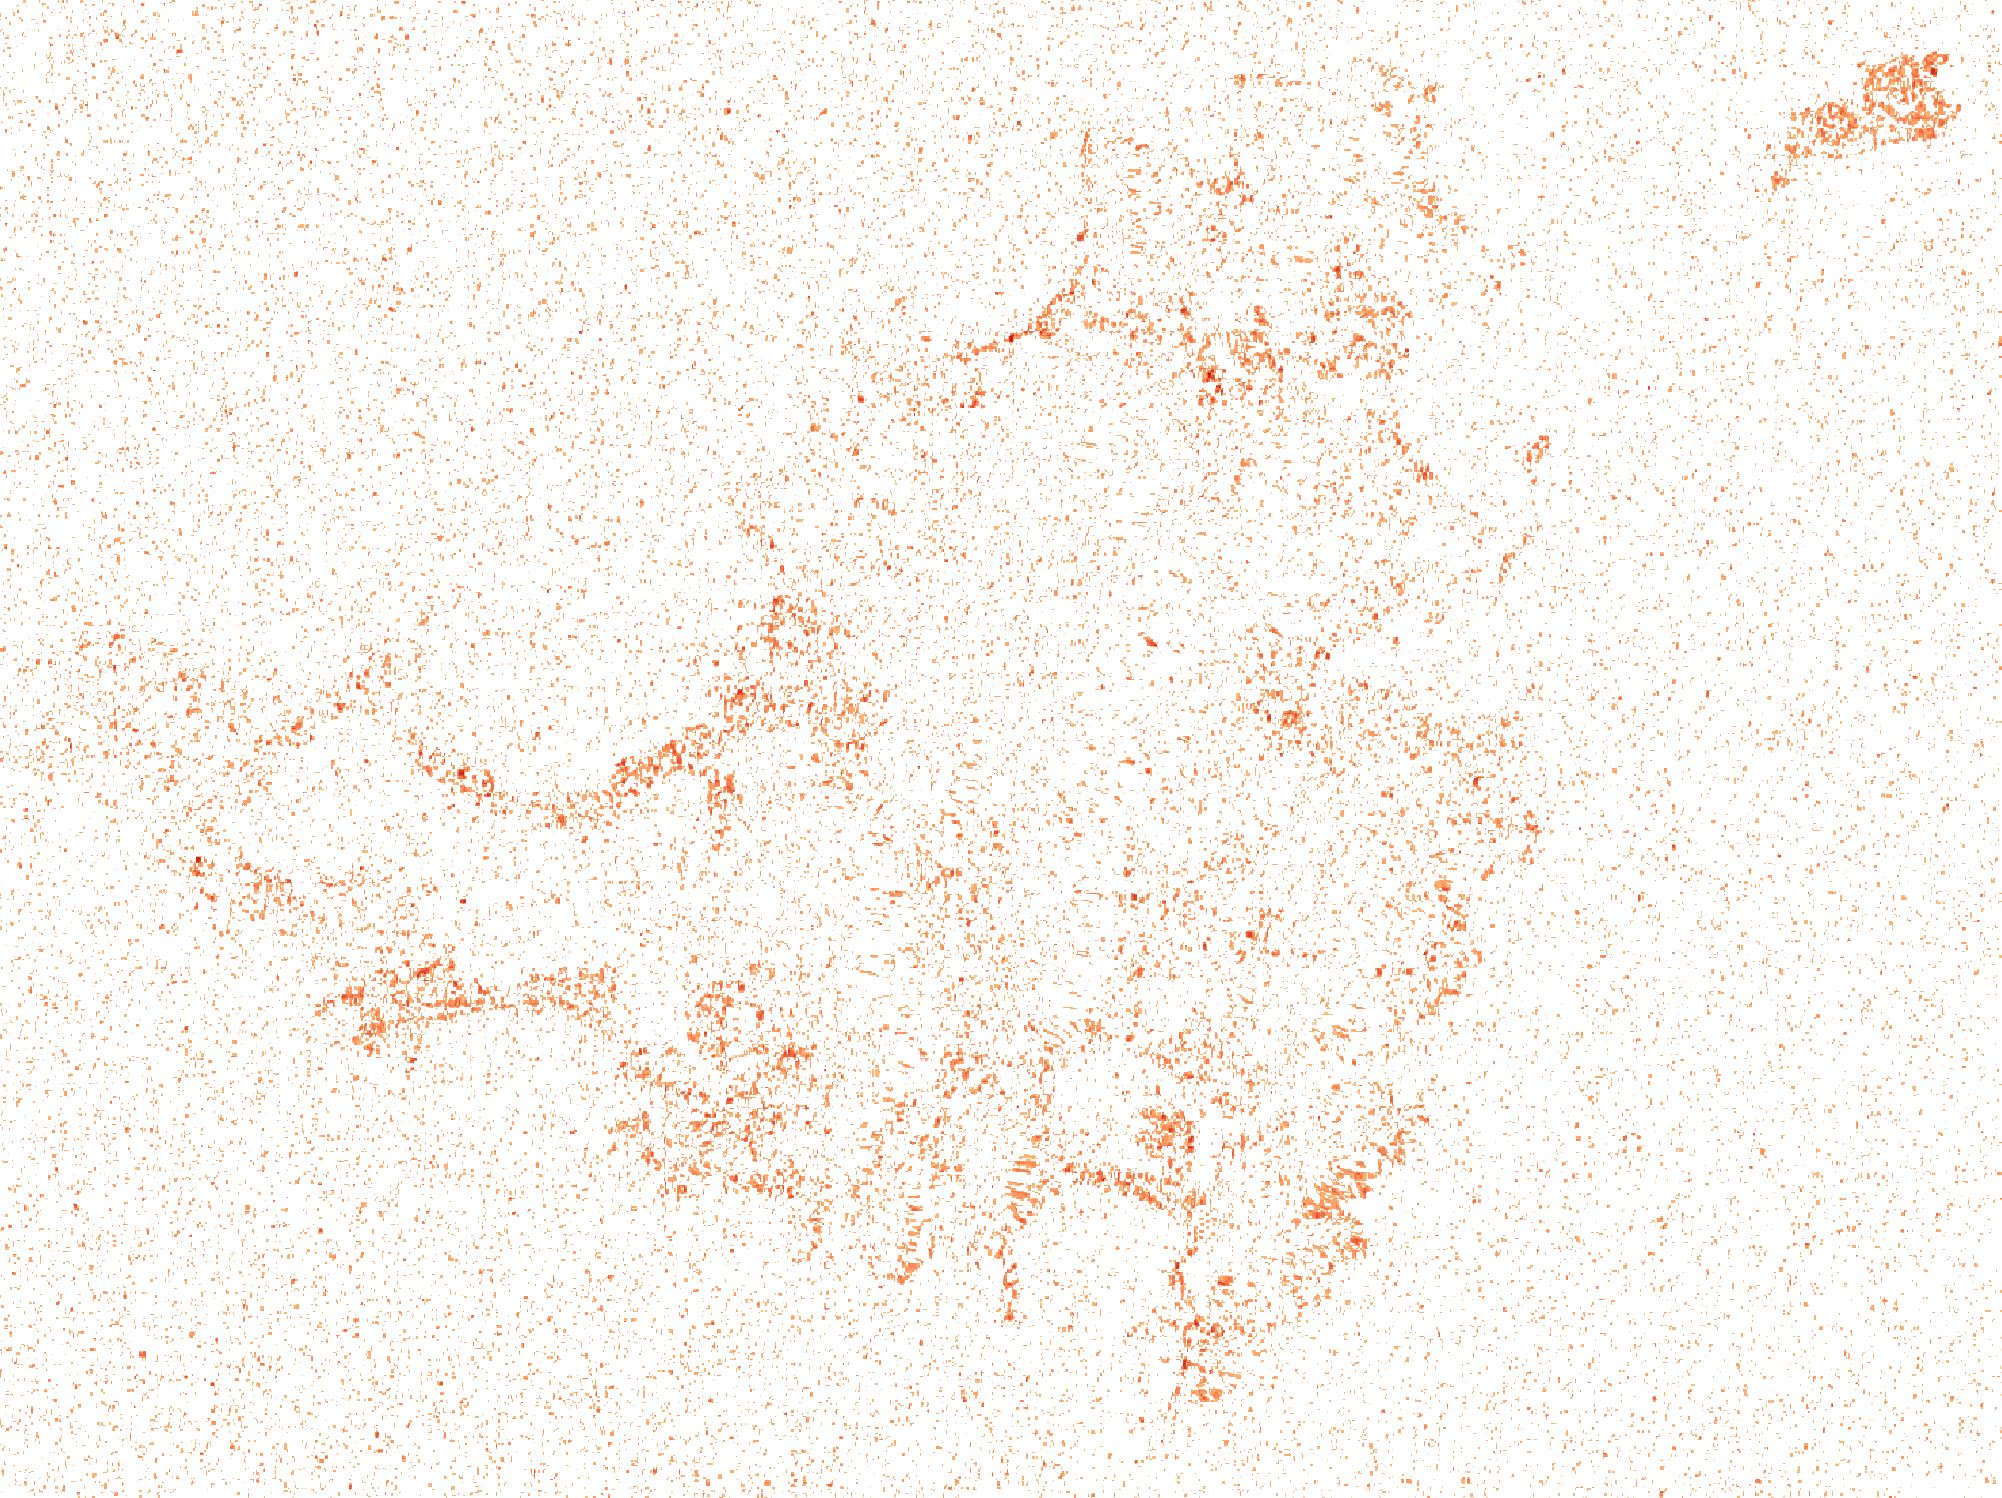
\includegraphics[width=0.95\textwidth]{figs/IntThres_03.png}
	\caption{\footnotesize{Result from empirically set threshold [0.3] after Univariate Image Differencing from the coherence maps. Darker colour indicate more change. All change under the threshold has been discarded and pixels are considered not damaged.}}
	\label{fig:YunOut}
\end{figure}

\subsection{Optical data}
The \ac{uav} dataset for Middle Region from RescUAV and aerial imagery from IGN have been used for the implementation of the \ac{eso} approach. To achieve a satisfactory result, the pre-event imagery has to be of the same geographic dimensions as the post-event imagery both as bounding box and concave hull. This to ensure the equalisation algorithm only affects -real- data and not the masked out areas. Figure \ref{fig:MidHSV} shows the characteristic non-rectangular outline from stitched \ac{uav} data. The correct pre-event dataset was created by using a mask with the outline of the post-event data from the \ac{uav}. This was done with the following steps:

\begin{itemize}
	\item For every pixel in the post-event imagery, it was decide if this pixel had data, if so it was classified as 1, otherwise 0.
	\item The resulting raster was vectorised to create a mask of the area.
	\item The polygon with value 0 was discarded.
	\item Using the polygon with value 1 a comparable pre-event dataset was created from the aerial imagery\\
\end{itemize} 

\noindent However, the first results show an error in the geographic alignment of the pre-event and post-event data [Figure \ref{fig:all}]. There is a very apparent shift in the datasets, this could be caused by various sources. As can be seen in figure \ref{fig:all}, the shift is not of the same magnitude throughout the image. The pool on the right hand side of the imagery has moved further than the buildings on the left hand side of the imagery. One explanation would be an error in the geo-referencing algorithm that stitched either the pre-event or post-event data. However, it is more likely that the \ac{uav} data has a lower accuracy in positioning than the aerial imagery used. This could cause the uneven shift throughout the image. To continue the research, some [four] of the datasets have been manually geo-referenced, using rubber-sheeting algorithms in Qgis, based on the pre-event aerial imagery available. These areas are Middle Region, Cul du Sac, St. Peters East, and Billy Folly.\\

\begin{figure}[!h]
	\centering
	\captionsetup{justification=raggedright,singlelinecheck=false}
	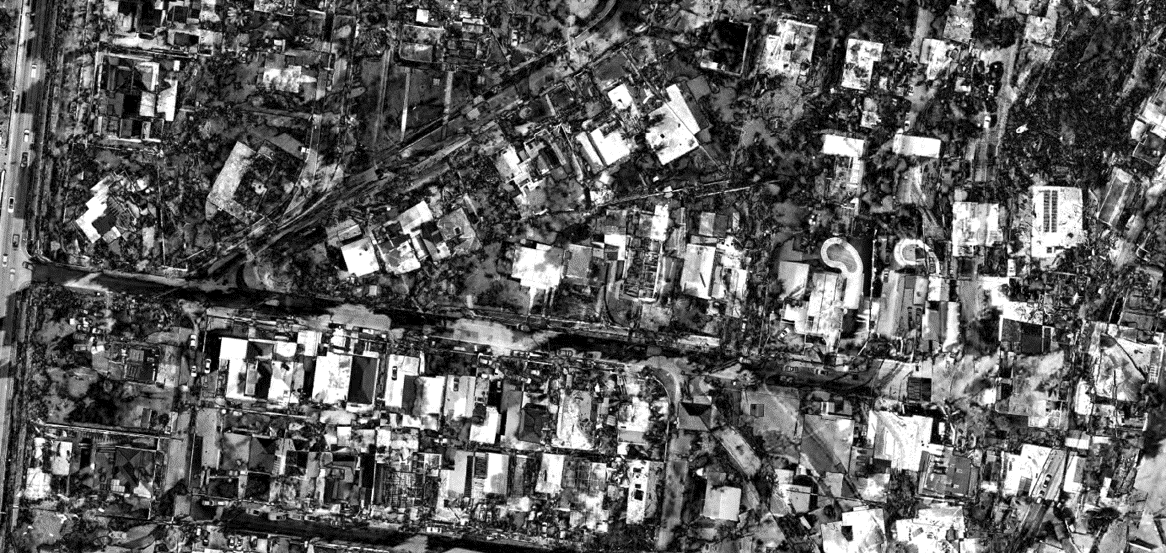
\includegraphics[width=0.85\textwidth]{figs/allignment.png}
	\caption{\footnotesize{Result of univariate image differencing before rubber-sheeting for geo-referencing.}}
	\label{fig:all}
\end{figure}

\noindent From the creation of these dataset the method as described in \ref{sec:Myun} could be implemented. For Middle Region all three characteristic bands where calculated and went through the histogram matching and univariate image differencing algorithm. All with varying results. In figure \ref{fig:MidComp} the results are visually compared to the original \ac{rgb} image. From this comparison it can be concluded that the use of lightness, equalised relative to the pre-event situation allows for the best manual interpretation of the data. However, this is due to the capabilities for humans to build connections and recognise objects in abstract representations of data, section \ref{sec:comp} will quantify the results. The lighter colour implies more change, in the hue change map nearly all buildings are a lighter colour indicating that something else is causing the change. The same amounts for saturation in which non of the buildings seem to have undergone significant change, while this is certainly the case. The value layer is not a perfect one-to-one indication of damage to building, however it does indicate change on the buildings which have sustained damage. This is specifically true in the cohesion of the pixels within the feature, not specifically on their intensity.

\begin{figure}[!h]
	\centering
	\captionsetup{justification=raggedright,singlelinecheck=false}
	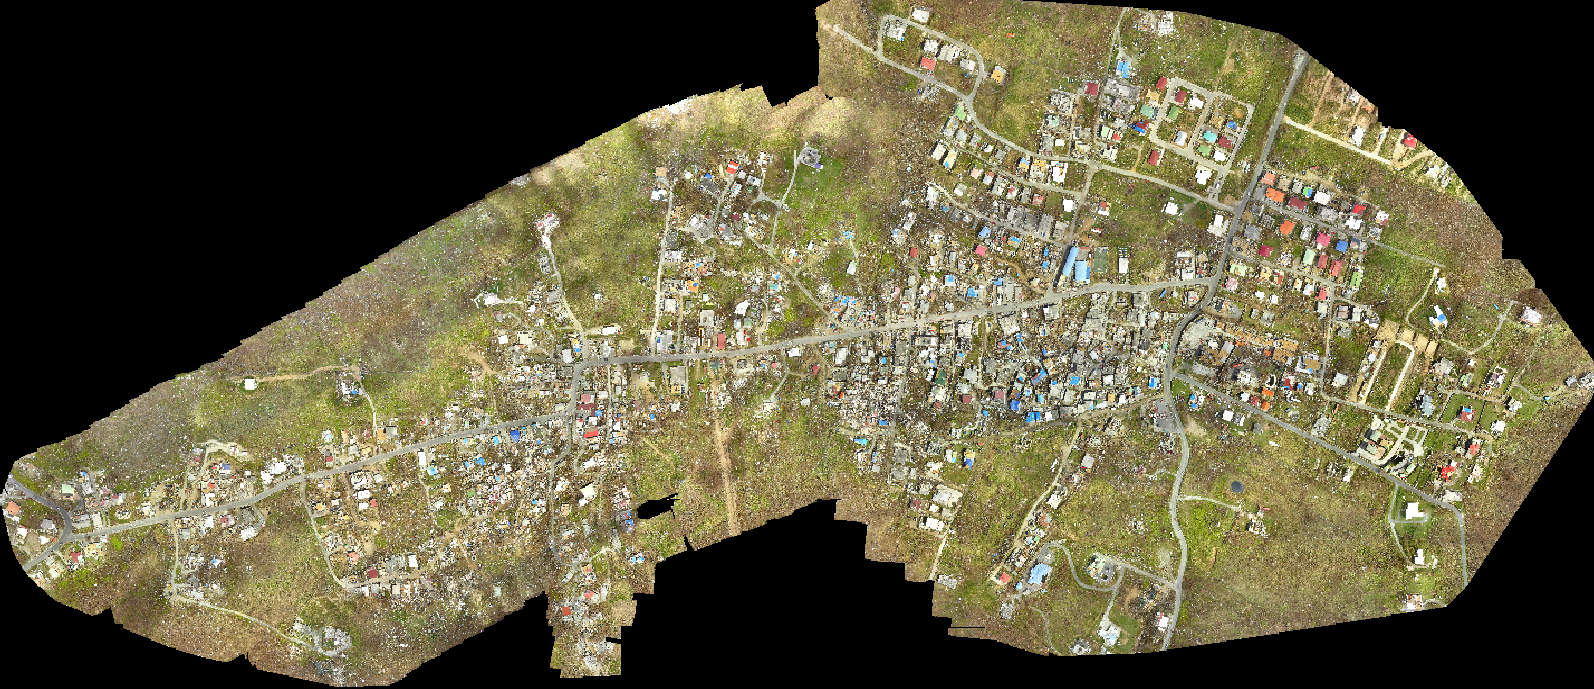
\includegraphics[width=0.85\textwidth]{figs/DataSetMid.png}
	\caption{\footnotesize{Optical \ac{uav} imagery Middle Region, with masked extent [From: RescUAV (17 Sept. 2017), Middle Region - Sint Maarten [georeferenced image], used under CC-BY4.0 as part of Open Imagery Network, retrieved from \url{www.openaerialmap.org}]}}
	\label{fig:MidHSV}
\end{figure}

 \begin{figure}[h]
	\centering
	\captionsetup{justification=raggedright,singlelinecheck=false}
	\begin{subfigure}{.8\textwidth}
		\centering
		\includegraphics[width=.95\linewidth]{figs/HistAfter.png}
		\caption{\footnotesize{Raw data}}
	\end{subfigure}
	\begin{subfigure}{.8\textwidth}
		\centering
		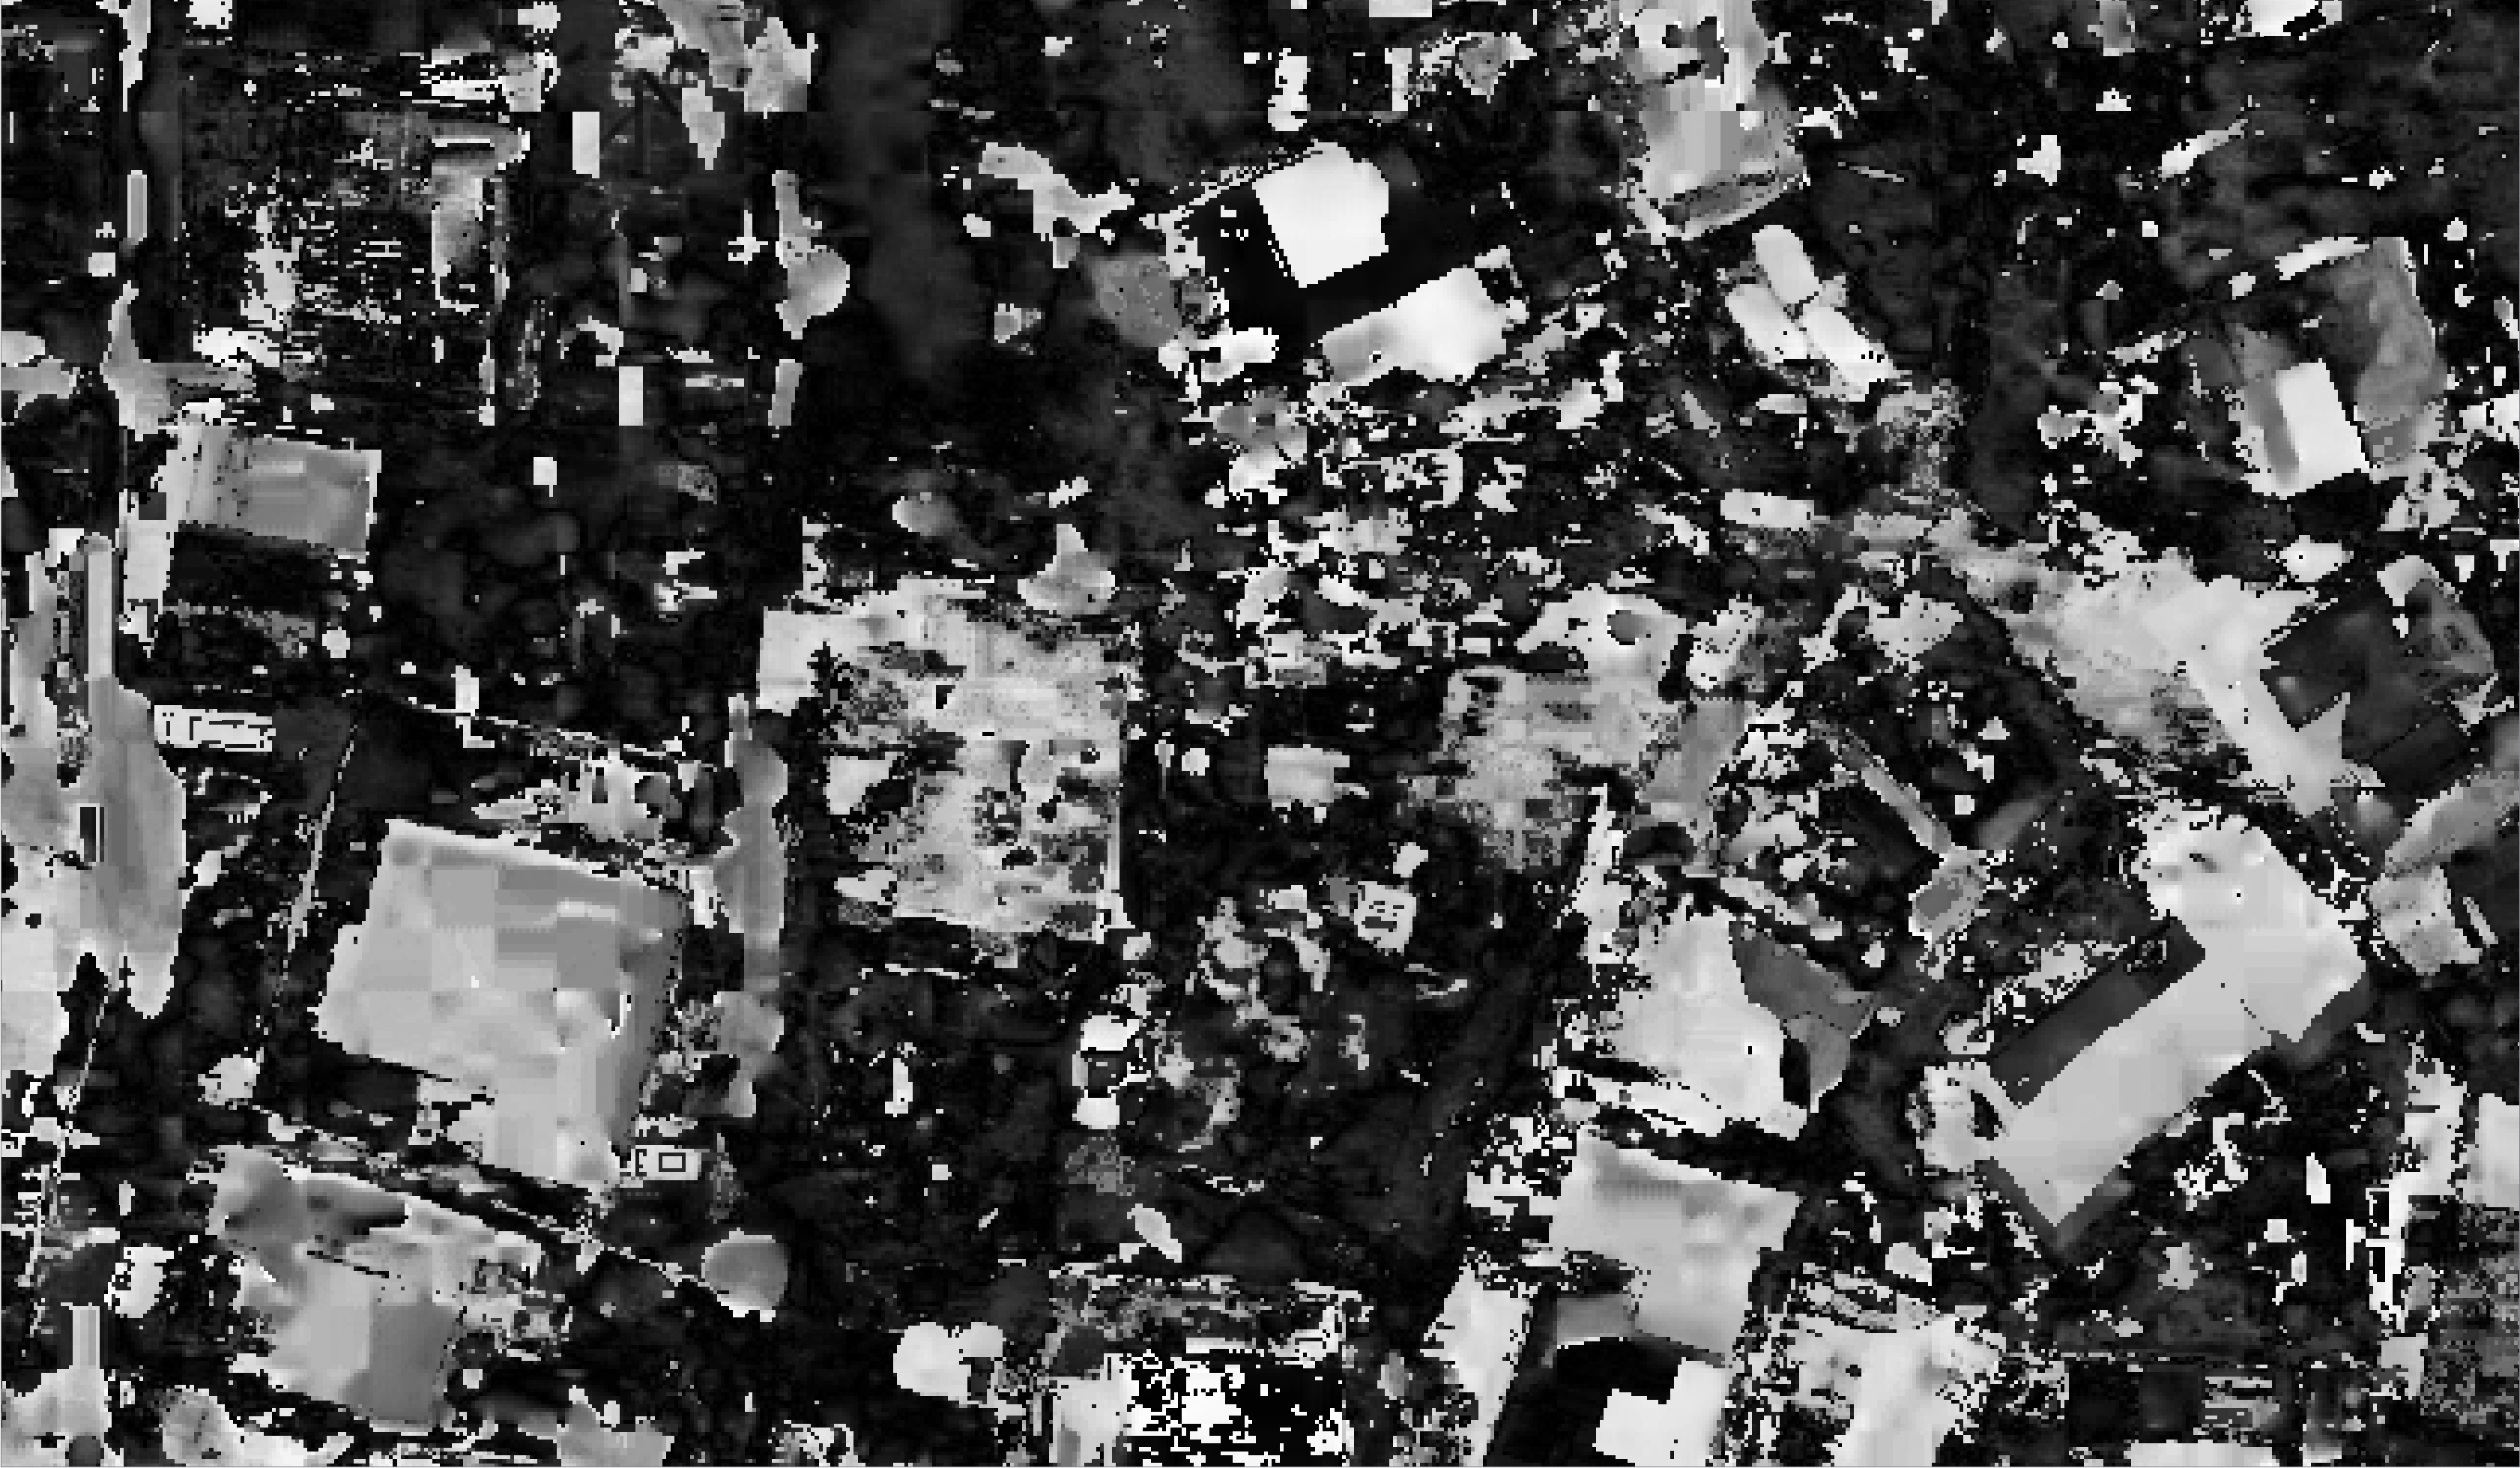
\includegraphics[width=.95\linewidth]{figs/HhistMid.png}
		\caption{\footnotesize{Hue change map}}
	\end{subfigure}
	\begin{subfigure}{.8\textwidth}
		\centering
		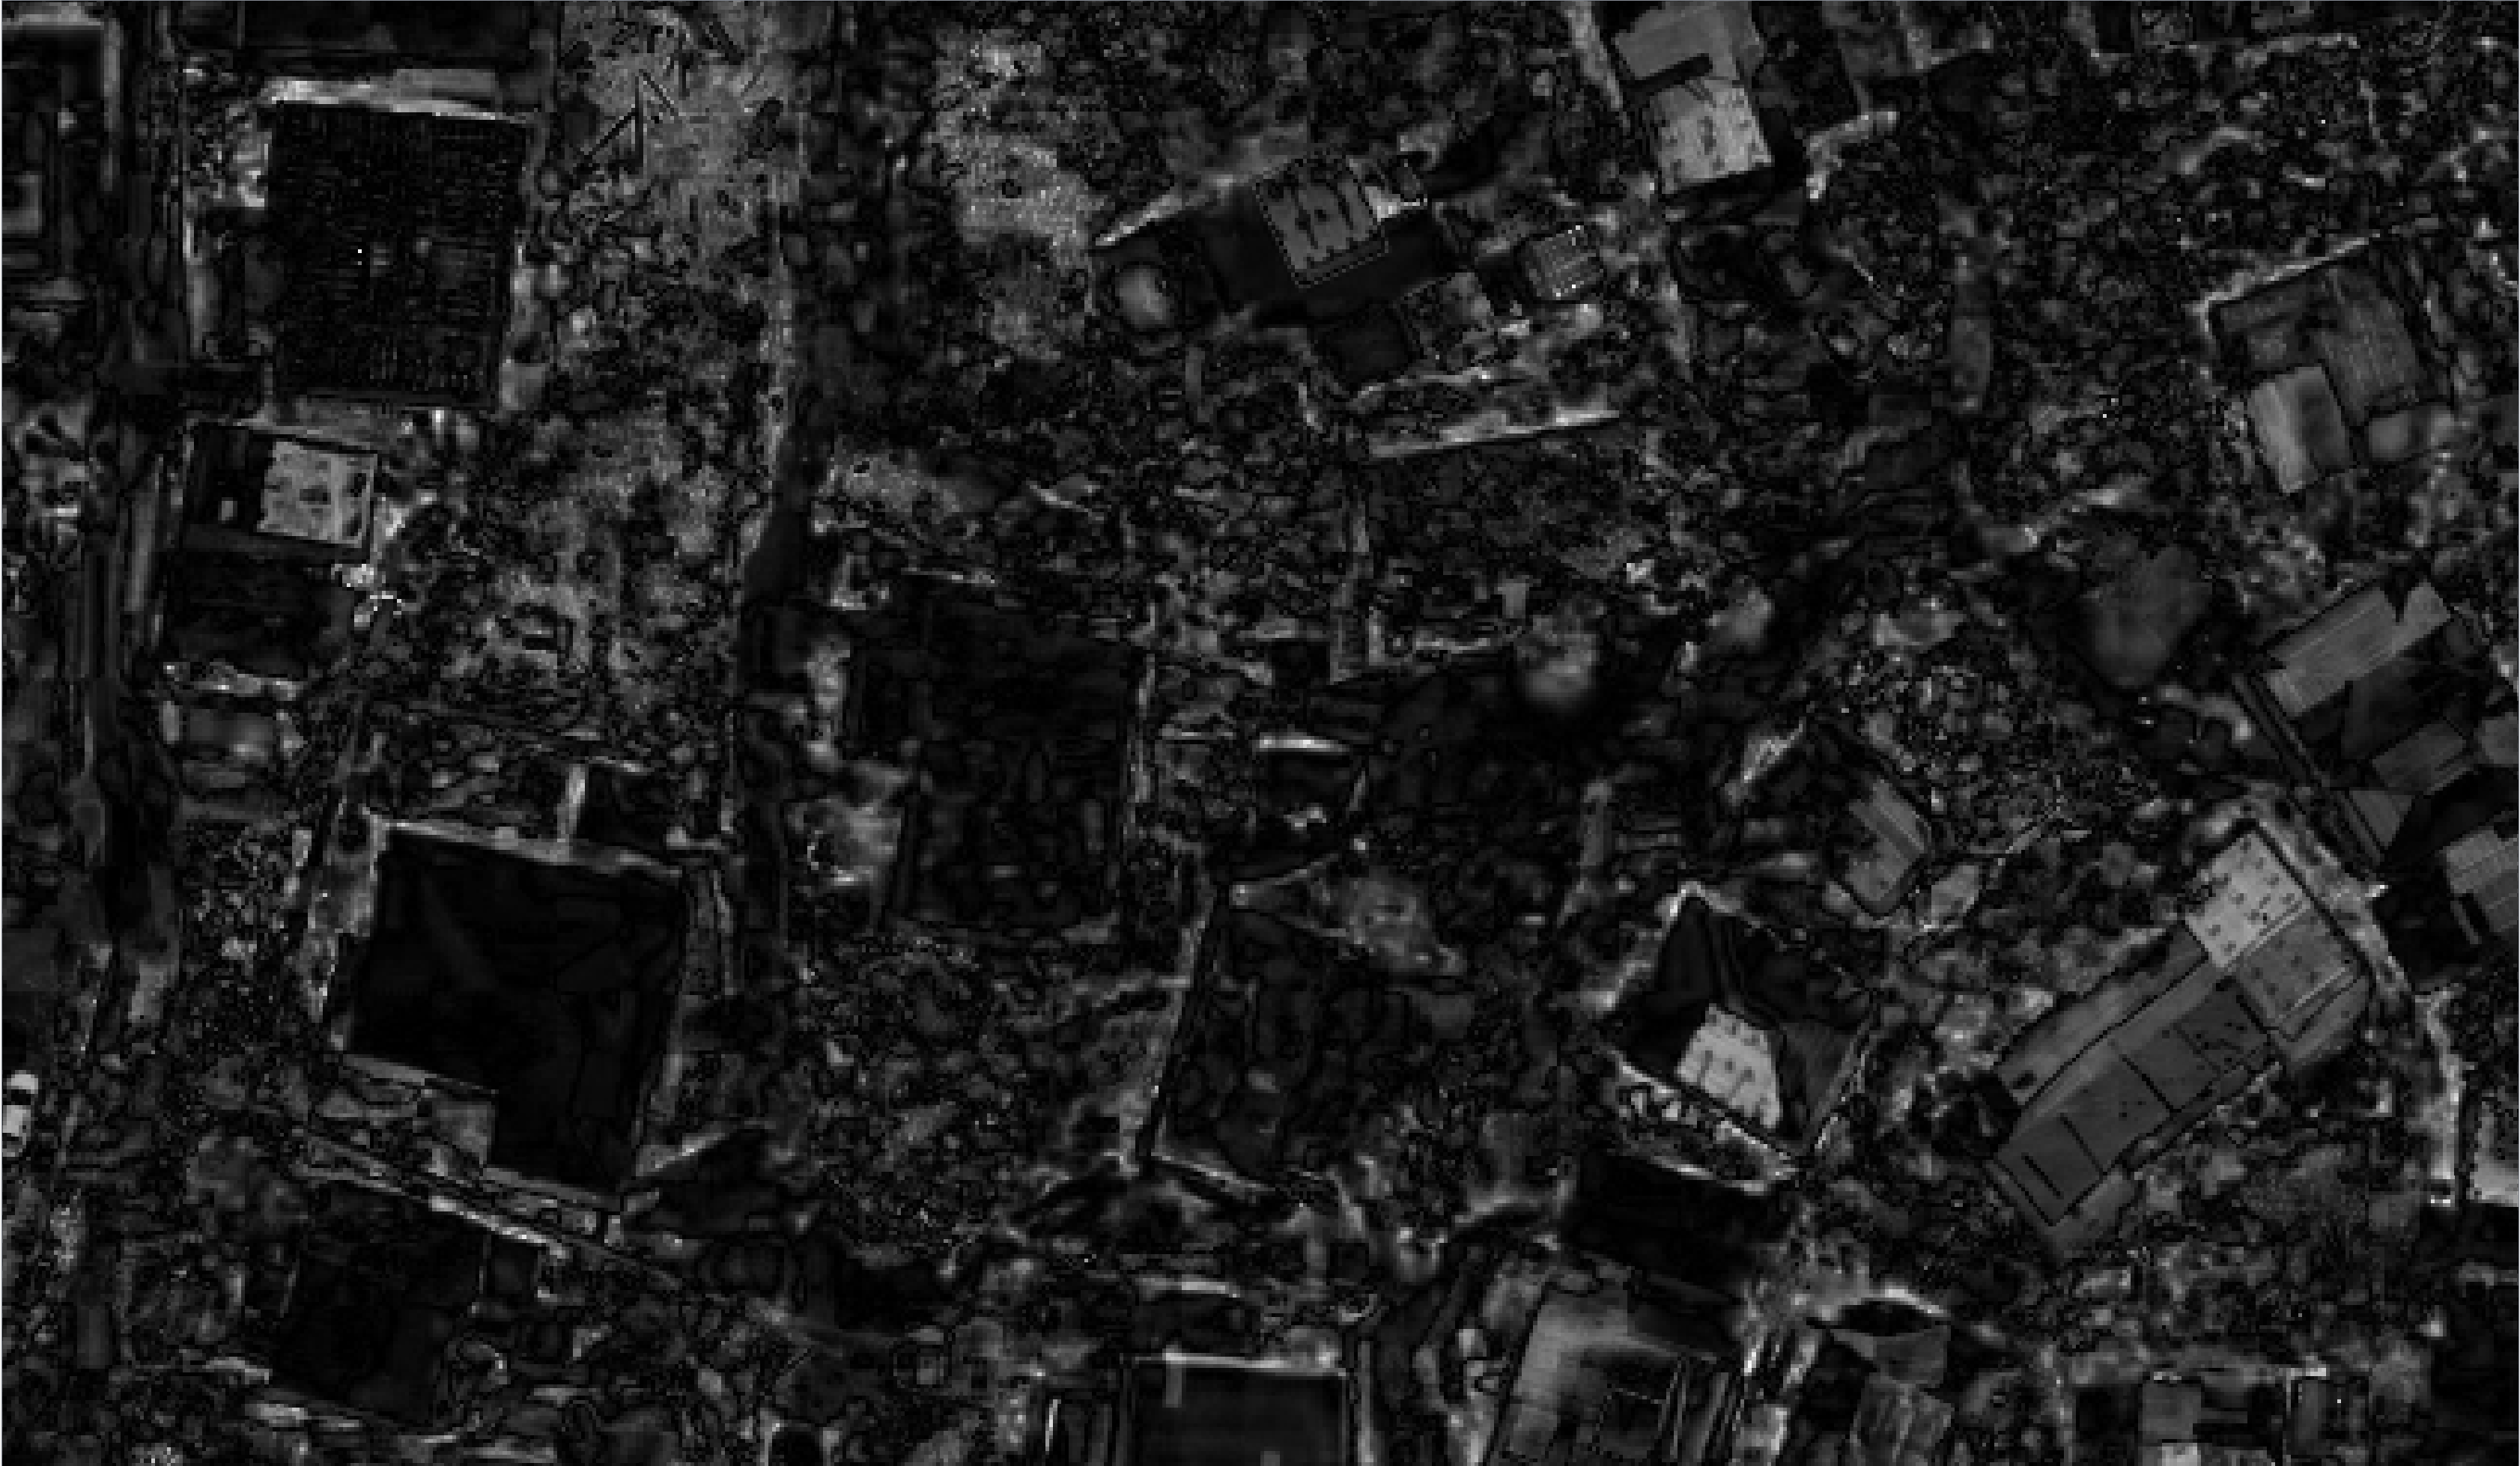
\includegraphics[width=.95\linewidth]{figs/ShistMid.png}
		\caption{\footnotesize{Saturation change map}}
	\end{subfigure}
	\begin{subfigure}{.8\textwidth}
	\centering
	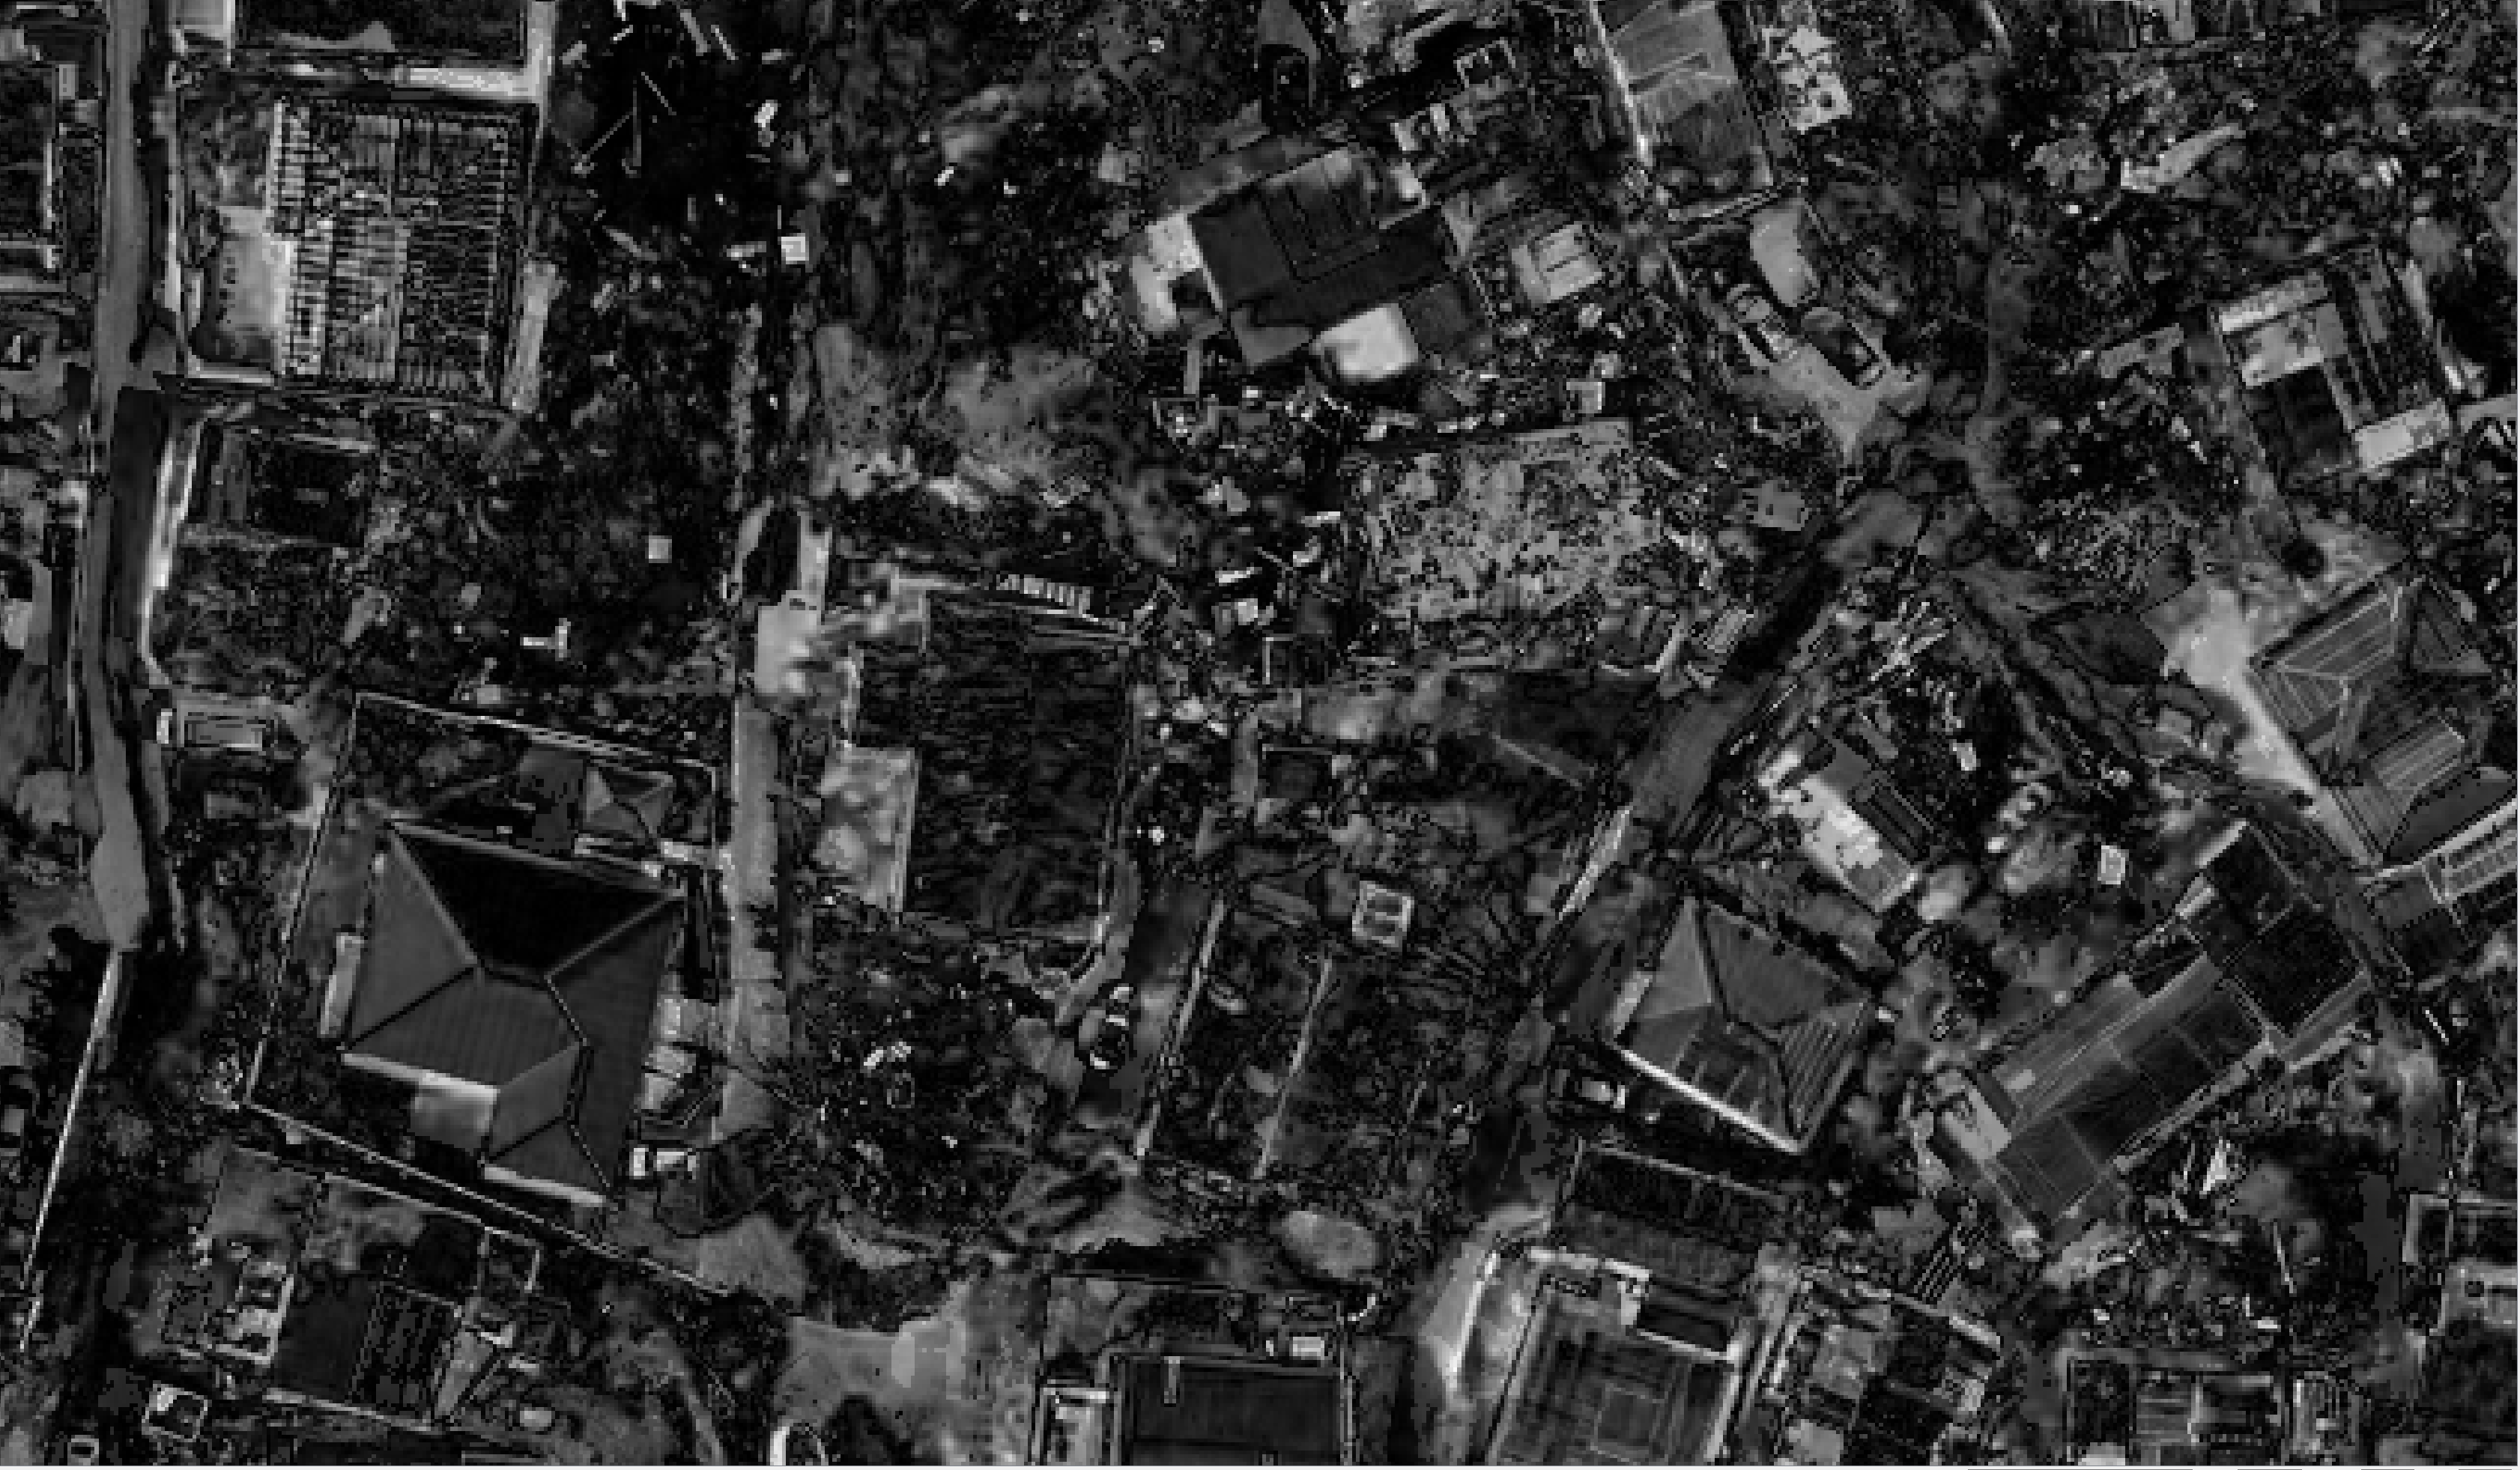
\includegraphics[width=.95\linewidth]{figs/VhistMid.png}
	\caption{\footnotesize{Value change map}}
	\end{subfigure}
	\caption{\footnotesize{Comparison between Dataset Middle Region on a normalised scale. [From: RescUAV (17 Sept. 2017), Middle Region - Sint Maarten [georeferenced image], used under CC-BY4.0 as part of Open Imagery Network, retrieved from \url{www.openaerialmap.org}]}}
	\label{fig:MidComp}
\end{figure}
\clearpage
\section{Convolutional Neural Network} \label{sec:Rvet}
\subsection{Optical data} \label{sec:cno}
As described in section \ref{sec:Mvet} there are three steps necessary for the creation of a \ac{cnn} method. First of all the features need to be created. In the case of St. Maarten these features can be created from available data. The square bounding boxes necessary for a fruitful implementation of a \ac{cnn} was done using features, with classification from OpenStreetMap. These bounding boxes where than used to cut features of 100x100 pixels from the various input layers. These layers are the \ac{uav} datasets, which have been used for the creation of the ground truth data; which is the foundation of the \ac{cnn}. A sample of these features have been represented in figure \ref{fig:features}. From this image it can already be noted that not all of the features have been selected correctly. This is mainly due to the geographical shift between images from before and after the disaster. As described in section \ref{sec:Ryun} this shift has a varying magnitude through out the datasets and can only be fixed by rubber-sheeting geo-referencing. Due to the time constraints of this research, these transformations where not possible. Hence an attempt has been done with the available data.\\

\begin{figure} [H]
	\centering
	\captionsetup{justification=raggedright,singlelinecheck=false}
	\begin{subfigure}{.275\textwidth}
		\centering
		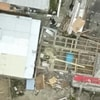
\includegraphics[width=.95\linewidth]{figs/1.jpg}
	\end{subfigure}
	\begin{subfigure}{.275\textwidth}
		\centering
		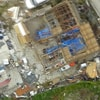
\includegraphics[width=.95\linewidth]{figs/2.jpg}
	\end{subfigure}
	\begin{subfigure}{.275\textwidth}
		\centering
		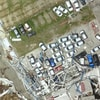
\includegraphics[width=.95\linewidth]{figs/3.jpg}
	\end{subfigure}
	\par\medskip
	\begin{subfigure}{.275\textwidth}
		\centering
		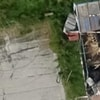
\includegraphics[width=.95\linewidth]{figs/4.jpg}
	\end{subfigure}
	\begin{subfigure}{.275\textwidth}
		\centering
		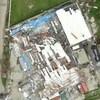
\includegraphics[width=.95\linewidth]{figs/5.jpg}
	\end{subfigure}
	\begin{subfigure}{.275\textwidth}
		\centering
		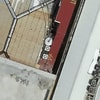
\includegraphics[width=.95\linewidth]{figs/6.jpg}
	\end{subfigure}	
	\par\medskip
	\begin{subfigure}{.275\textwidth}
		\centering
		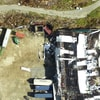
\includegraphics[width=.95\linewidth]{figs/7.jpg}
	\end{subfigure}
	\begin{subfigure}{.275\textwidth}
		\centering
		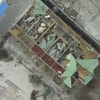
\includegraphics[width=.95\linewidth]{figs/8.jpg}
	\end{subfigure}
	\begin{subfigure}{.275\textwidth}
		\centering
		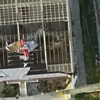
\includegraphics[width=.95\linewidth]{figs/9.jpg}
	\end{subfigure}

	\caption{\footnotesize{Features generated from bounding boxes, classified as destroyed}}
	\label{fig:features}
\end{figure}

\noindent The \ac{cnn} architecture described in \ref{sec:Myun} has been implemented in TFlearn for Python and run on the available dataset. This run is based on the settings from \citet{Vetrivel2016b} and implemented for damage detection. The first training was based on a learning rate of 0.1, 5 epochs, and no normalisation. Unfortunately where the first runs unsuccessful with over-fitting of the regression layer. This resulted in a varying loss indicator, but a stable validation accuracy. To avoid over-fitting more epoch where run with the same settings. A slow increase to 5, 10, 15, 25, and 35 epoch had no influence on the results. Over-fitting was the norm and no to little increases in the loss function or accuracy where noted. A similar approach was used for the increase of the learning rate from 0.1 to 0.01, with similar results. The addition of normalisation should allow for a better distribution of the features, resulting in better predictability. However, after 35 epochs [figure \ref{fig:epoch}] the neural network still over-fits. The resting validation accuracy can be interpreted as the regression layer continually predicting the same class, the validation accuracy in this case therefore arises from the fact that guessing this option gives the best outcome most of the time. This is the result of a skewed input regarding the classes, or skewed input regarding the actual features. 

\begin{figure} [H]
	\centering
	\captionsetup{justification=raggedright,singlelinecheck=false}
	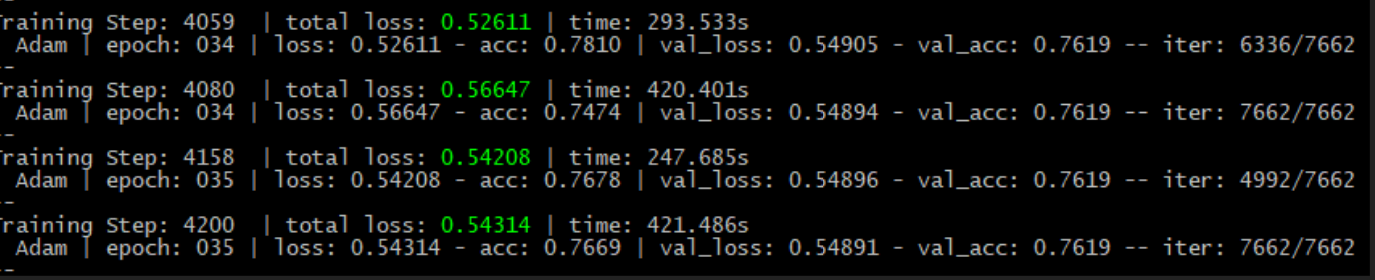
\includegraphics[width=0.95\textwidth]{figs/Epoch3435.png}
	\caption{\footnotesize{Training of \ac{cnn}, last 2 epochs, full training in appendix \ref{an:key}}}
	\label{fig:epoch}
\end{figure}

\subsection{\ac{sar} data} 
The characteristics of the \ac{sar} data do not allow for the use of a \ac{cnn} method. As described in section \ref{sec:vet} for a \ac{cnn} to work it needs to do convolutions on the datasets. As shown in figure \ref{fig:sarbui} the pixel size of the \ac{sar} dataset is of the same magnitude as the building outlines. This results in less than 1 pixel per structure, thus per feature. A \ac{cnn} can not perform any convolutions or other transformations on a feature that starts with only one pixel value. This would not allow for the detection of borders or other characteristics which might encompass change or damage. A machine learning approach could still be feasible, however this would now be focussed on a 1D feature vector, comparable to those of support vector machines or least squares adjustment. As these methods differ from a close comparison to the method proposed by \citet{Vetrivel2016b} these have not been considered in this research.
\begin{figure} [H]
	\centering
	\captionsetup{justification=raggedright,singlelinecheck=false}
	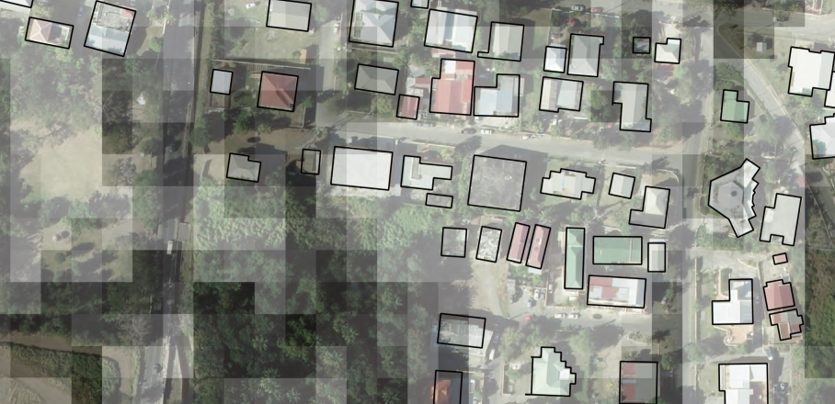
\includegraphics[width=0.95\textwidth]{figs/superim.png}
	\caption{\footnotesize{\ac{sar} coherence map superimposed on buildings [Based on: RescUAV (17 Sept. 2017), Middle Region - Sint Maarten [georeferenced image], used under CC-BY4.0 as part of Open Imagery Network, retrieved from \url{www.openaerialmap.org}]}}
	\label{fig:sarbui}
\end{figure}
\section{Comparison} \label{sec:comp}
From sections \ref{sec:Ryun} and \ref{sec:Rvet} the matrix from section \ref{sec:prep} can be filled. Matrix \ref{tab:matrConc} indicates which methods have been tested and which was not possible to execute. However, some implementations so far have been focused on visual interpretation as a last step in determining damage. This section will quantify the results for a direct comparison on accuracy performance for damage detection as described in section \ref{sec:clas}. The extension and comparison of the methods is described in section \ref{sec:ext}.\\
\begin{table} [h]
	\centering
	\captionsetup{justification=raggedright,singlelinecheck=false}
	\caption{\footnotesize{Matrix used for comparison methods and data, Green = Implemented, Orange = Not implemented.}}
	\begin{footnotesize}
		\begin{tabular}{m{2.5cm}|m{2.5cm}|m{2.5cm}|}
			\cline{2-3}
			& Optical \ac{uav} Data & Satellite \ac{sar} Data \\ \cline{2-3}
			Equalisation and subtraction & \cellcolor{JungleGreen!30} \ac{eso} & \cellcolor{JungleGreen!30} \ac{ess} \\ \hline
			Convolutional Neural Network & \cellcolor{JungleGreen!30} \ac{cno} & \cellcolor{orange!30} \ac{cns} \\ 
			\hline
		\end{tabular}
	\end{footnotesize}
	\label{tab:matrConc}
\end{table}

\noindent The quantification for the \ac{eso} and \ac{ess} is done by empirically checking various possible combinations of thresholds and feature statistic and the calculation of the Cohen Kappa Coefficient. Only a summary of these results with the highest Cohen Kappa coefficient will be compared, these are fully represented in appendix \ref{an:coh}. For the \ac{cno} approach, the network as described in sections \ref{sec:vet} and \ref{sec:Mvet} is trained on all data available expect Middle Region. This pre-trained network is then used for the detection of damage in the features from Middle Region. Lastly the \ac{stoa} method, implemented by Copernicus \ac{ems} is considered and compared. All of these results are available in table \ref{tab:eso}.\\

\noindent The ground truth data consist out of vector representations of the buildings on the island and their respective classification as described in section \ref{sec:clas}. To allow fair comparison between this data and the other methods for damage detection this datasets will need to be translated to match the granularity of the damage description. In this case, four categories have been reduced to two. These classes have been used in the comparison between methods described in this section. Table \ref{tab:clastrans} shows this reduction translation between classes.\\

\begin{table} [H]
	\centering
	\footnotesize
	\captionsetup{justification=raggedright,singlelinecheck=false}
	\caption{\footnotesize{Translation from damage classification provided in ground truth to damage detection, as defined in section \ref{sec:clas}}}	
	\begin{tabular}{ll}
		\toprule
		Damage classification & Damage Detection \\
		\midrule			
		No Damage &\\
		Minimal Damage & No Damage\\
		\midrule	
		Significant Damage &\\
		Critical Damage & Damage\\
		\bottomrule
	\end{tabular}
	\label{tab:clastrans}
\end{table} 

\noindent For the \ac{eso} and \ac{ess} approaches four change maps, namely the interferometry and \ac{hsv} change sets from the \ac{uav} optical data, are considered. To do so these pixel values have been aggregated over the various buildings outlines. These vector representations of the buildings are derived from the ground truth data. By subsequently taking the median of intersecting or enclosed pixels an aggregated value is derived per building. To determine whether a building is damaged a threshold needs to be empirically set to differentiate between damaged buildings and non damaged buildings. Such a threshold is determined for all four changes maps systematically. These have been generated for every 0.01 of change within the change maps, resulting in one hundred thresholds per image. All quantifications are then compared to the ground truth data obtained by visual interpretation by the \ac{nlrc}. Table \ref{tab:eso} summarise the best findings, based on their Cohen Kappa Scores. In appendix \ref{an:coh} the full F1 matrices, and confusion matrices from the four change maps are represented. From that table \ref{tab:eso} it can be concluded that although the method is working, it is not on the data for which it is intended. The interferometry data has a low Kappa score and F1-score of 0.45, this is about comparable to estimated guessing with a-priori knowledge of the damage distribution. For the optical approaches, namely Saturation and Value, the empirical threshold does allow for better results especially considering regarding the considerations saturation and value, even though these might not have seem a direct hit on visual interpretation, they do provide knowledge about the distribution of damage, with both Cohen Kappa scores around the 0.5 and F1-scores close to 0.7. Furthermore, both perform well on the detection of damage, for which the F1-scores are 0.74 and 0.73 respectively.\\

\noindent  As mentioned in section \ref{sec:cno} the \ac{cno} approach fails to converge on the loss indicator. This is due to the skewed input as a result of geographic misalignment. Therefore, all features have been classified as not damaged, as shown in the confusion matrix in table \ref{tab:confcno}. This is reflected in the indices for both F1-score and Cohen Kappa coefficient [Table \ref{tab:clastrans}]. 

\begin{table} [H]
	\centering
	\footnotesize
	\captionsetup{justification=raggedright,singlelinecheck=false}
	\caption{Confusion matrix [Vertical Ground Truth, Horizontal predicted] for the \ac{cno} based method. }	
	\begin{tabular}{l|llll}
		& No    & Damage & unknown &  \\ \hline
		No      & 519.0 & 0.0    & 0.0     &  \\
		Damage  & 321.0 & 0.0    & 0.0     &  \\
		unknown & 16.0  & 0.0    & 0.0     &  \\
	\end{tabular}
\label{tab:confcno}
\end{table}

\noindent Lastly, the \ac{stoa} method implemented by Copernicus \ac{ems} was compared to the ground truth. As with the ground truth, the \ac{stoa} data are vector representations of the buildings with classifications attached. The \ac{stoa} data has been spatially matched to the vector representations of the ground truth data, to ensure the vector representations corresponded to the right classifications in both methods. Like with the ground truth data, the \ac{stoa} classifications need to be translated to damage detection, table \ref{tab:clastrans2} shows the corresponding categories. From the comparison and corresponding confusion matrix [Table \ref{tab:confcop}], using the same accuracy measurements for agreement as the other methods, it can be concluded that the \ac{stoa} approach heavily overestimates the damage. It is also indicated that the method does not significantly outperform other methods implemented in this research.  

\begin{table} [H]
	\centering
	\footnotesize
	\captionsetup{justification=raggedright,singlelinecheck=false}
	\caption{\footnotesize{Translation from damage classification provided in the \ac{stoa} method to damage detection, the latter as defined in section \ref{sec:clas}}}	
	\begin{tabular}{ll}
		\toprule
		Damage classification & Damage Detection \\
		\midrule			
		Not affected &\\
		Negligible to slight Damage & No Damage\\
		\midrule	
		Moderately Damaged &\\
		Highly Damaged & \\
		Completely Destroyed & Damage\\
		\bottomrule
	\end{tabular}
	\label{tab:clastrans2}
\end{table} 

\begin{table} [H]
	\centering
	\footnotesize
	\captionsetup{justification=raggedright,singlelinecheck=false}
	\caption{Confusion matrix [Vertical Ground Truth, Horizontal predicted] for the \ac{stoa} approach. }	
	\begin{tabular}{l|llll}
		& No    & Damage & unknown &  \\ \hline
		No      & 142.0 & 377.0  & 0.0     &  \\
		Damage  & 51.0  & 270.0  & 0.0     &  \\
		unknown & 4.0   & 12.0   & 0.0     &  \\
	\end{tabular}
	\label{tab:confcop}
\end{table}

\begin{table} [H]
	\centering
	\footnotesize
	\captionsetup{justification=raggedright,singlelinecheck=false}
	\caption{\footnotesize{Accuracy comparison between methods described in chapter \ref{implem}, quantified using thresholds and ground truth data.}}	
	\begin{tabular}{llll}
		\toprule
		Technique & Threshold & Kappa coeff. & Avg. F1-Score \\
		\midrule			
		\ac{eso} Hue & 0.11 & 0.070 & 0.47\\
		\ac{eso} Saturation & 0.07 & 0.429 & 0.71\\
		\ac{eso} Value & 0.21 & 0.389 & 0.69\\
		\ac{ess} & 0.30 & 0.059 & 0.54\\
		\midrule
		\ac{cno} & n/a & 0.000 & 0.46\\
		\midrule
		\ac{stoa} & n/a & 0.093 & 0.45\\
		\bottomrule
	\end{tabular}
\label{tab:eso}
\end{table} 
\section{Extension to classification} \label{sec:ext}
To answer the main research question fully, an evaluation of the extended methods for classification is indispensable. The implementation for extension require little change to the existing methods and is based on the same principles. The definition for classification of damage as described in section \ref{sec:clas} is used. Therefore, the ground truth data is used without translation as it is already based on this definition. To facilitate the extension of the \ac{eso} and \ac{ess}, multiple thresholds are required. As in section \ref{sec:comp}, these threshold will be systematically empirically checked. With the four classes defined for damage classification this translates to three thresholds. The extension of the \ac{cno} approach requires little tweaking of the deepest, regression layer of the \ac{cnn}, in which the parameters are tuned from two to four classes. The \ac{stoa} classification still differentiates from the defined classification and requires a translations schema. The summary of the results is presented in table \ref{tab:extended}.\\

\noindent For the systematic approach to the three thresholds for the \ac{eso} and \ac{ess} methods, all valid combinations of thresholds is examined. Intervals between thresholds are defined by 0.025 steps between 0 and 1, a combination of thresholds is considered valid when the third threshold is larger than the second threshold, which has to be larger than the first threshold. From all valid thresholds, those with the highest Cohen Kappa score are represented in table \ref{tab:clastrans3}.\\

\noindent The \ac{cno} approach has similar steps as in section \ref{sec:comp}. Through these steps, the network is retrained with the deepest layer altered for four classification categories, and this trained network is applied to the unseen dataset. However, as in the comparison for damage detection, the \ac{cnn} does not converge on the loss indicator [Appendix \ref{an:nnclas} provides an overview of the training] and all features classified as not damaged.\\

\noindent As the \ac{stoa} approach to classification is defined differently than in this research, the data needs to be translated for comparison. The same vector outlines as in section \ref{sec:comp} have been used but with the translation provided in table \ref{tab:clastrans3}. The resulting accuracy indices indicate a bleak implementation. The \ac{stoa} approach heavily overestimates the damage, corroborated by the confusion matrix [Table \ref{tab:confcop2}], as in the damage detection.\\

\begin{table} [H]
	\centering
	\footnotesize
	\captionsetup{justification=raggedright,singlelinecheck=false}
	\caption{\footnotesize{Translation from damage classification provided in the \ac{stoa} method to damage classification as defined in section \ref{sec:clas}}}	
	\begin{tabular}{ll}
		\toprule
		Damage classification & Damage Detection \\
		\midrule			
		Not affected &\\
		Negligible to slight Damage & No Damage\\
		\midrule	
		Moderately Damaged & Partial Damage\\
		\midrule
		Highly Damaged & Significant Damage\\
		\midrule
		Completely Destroyed & Critical Damage\\
		\bottomrule
	\end{tabular}
	\label{tab:clastrans3}
\end{table} 

\begin{table} [H]
	\centering
	\footnotesize
	\captionsetup{justification=raggedright,singlelinecheck=false}
	\caption{Confusion matrix [Vertical Ground Truth, Horizontal predicted] for the \ac{stoa} approach for classification.}	
	\begin{tabular}{l|llll}
		& No    & Damage & unknown &  \\ \hline
		No      & 142.0 & 377.0  & 0.0     &  \\
		Damage  & 51.0  & 270.0  & 0.0     &  \\
		unknown & 4.0   & 12.0   & 0.0     &  \\
	\end{tabular}
	\label{tab:confcop2}
\end{table}

\begin{table} [H]
	\centering
	\footnotesize
	\captionsetup{justification=raggedright,singlelinecheck=false}
	\caption{\footnotesize{Accuracy comparison between methods described in chapter \ref{implem}, quantified using thresholds and ground truth data.}}	
	\begin{tabular}{llll}
		\toprule
		Technique & Threshold & Kappa coeff. & Avg. F1-Score \\
		\midrule			
		\ac{eso} Hue & 0.08, 0.11, 0.88 & 0.054 & 0.23\\
		\ac{eso} Saturation & 0.08, 0.08, 0.31 & 0.250 & 0.37\\
		\ac{eso} Value & 0.13, 0.18, 0.26 & 0.188 & 0.40\\
		\ac{ess} & 0.23, 0.31, 0.34 & 0.0511 & 0.30\\
		\midrule
		\ac{cno} & n/a & 0.00 & 0.21\\
		\midrule
		\ac{stoa} & n/a & 0.078 & 0.24\\
		\bottomrule
	\end{tabular}
	\label{tab:extended}
\end{table} 

\section{Discussion} \label{sec:disc}
This section provides discussion on the results from the comparison for damage detection and damage classification, as well as an interpretation of the framework for method assessment defined in section \ref{sec:framework}. The conclusions and recommendations from this discussion are presented in chapters \ref{concl} and \ref{reco} respectively.\\

\noindent The results gathered in sections \ref{sec:comp} and \ref{sec:ext} leave room for discussion and interpretation. First of all it must be noted that, as described in section \ref{sec:interrater}, the inter-rater statistics provide a tinted look on accuracy. However, agreement is considered a better description for accuracy in this case study. Although the extension of methods to damage classification is possible, they perform considerably less than the methods for damage detection. The main negative outliers in both approaches are the \ac{cno}, \ac{stoa}, and \ac{ess} approaches. As the results of the \ac{cno} approach are faulted by design, these are not considered for discussion. However, a lesson learned from this faulty approach is the need for properly geo-referenced imagery in the use of multiple datasets for damage determination, as corroborated in section \ref{sec:Ryun}. The bad performance in both damage classification as well as damage detection by the \ac{stoa} approach is unexpected. However, the speed with which these datasets are provided by UNOSAT or Copernicus \ac{ems} is nearly unbeatable as the first damage maps were available one week after the hurricane struck the island. Furthermore, this approach overestimates the damage in a disaster struck area, which is desirable for humanitarian organisations to ensure proficient aid is supplied. Lastly,the \ac{ess} approach is not suited for damage determination on a building scale level, however, this is also not claimed by \citet{Yun2015}. Therefore, this method might be unsuitable for building damage determination but it might still be useful in larger disaster where prioritisation of areas is paramount to an operation.\\

\noindent All methods considered, the \ac{eso} approach was the most surprising, as a deducted method from \citet{Yun2015}, it performs reasonable on a building scale level, mainly due to the increase in resolution. However, the empirically set threshold is not a robust approach for other disasters, as variations in camera systems or external influences might impact the performance. Ground truth data is therefore indispensable to make sure a threshold can be set systematically with a machine learning minimisation approach.\\

\noindent The implementations of the various methods and \ac{stoa} approach, have varying degrees of accuracy. However, accuracy is only one of the parameters defined in section \ref{sec:framework} for the assessments of methods for damage detection or classification. The others are acquisition time, acquisition method, and resolution for input data and output information. Acquisition time and acquisition method are highly depended and pros and cons have been summarised in table \ref{tab:edatasets}. The datasets used in this research are complementary, especially concerning the spatial coverage and resolution of input data. Most methods described in this research are able to provide output on a building level resolution, without regards to accuracy, and this is the required level of information for the phase from the \ac{drm} activity cycle on which this research focused. The \ac{sar} data is highly regular and can be provided within 6 days of a disaster indifferent of the atmospheric conditions, however the larger coverage area from this method is balance by the lower input resolution. Paired with the specialised technical know-how, and disappointing results in accuracy, this would not be the best implementation for the St. Maarten hurricane. In this specific disaster, the higher resolution input data from \ac{uav} imagery, provides more information than the larger extent, mainly due to the small size of the island. The methods used for optical imagery provide sufficient accuracy to be a better indication than \ac{stoa} approaches, and manual visual interpretation could provide ground truth information about the damage extent. 